\chapter{Referencial Teórico}\label{cap:refTeor}


Para se compreender a temática proposta, este capítulo abordará o conteúdo base deste trabalho dividido em 3 seções: Aprendizado de Máquina, Discretização e Trabalhos Correlatos. 

Essa primeira seção discorrerá sobre aprendizado de máquina e os aprendizados indutivos concedendo maior ênfase ao aprendizado supervisionado, em virtude da utilização de algoritmos de aprendizado supervisionado na rotulação de grupos, já na seção  \ref{cap:refTeor:sec:discret}, se dissertará sobre as técnicas de discretizações adotadas nesta pesquisa, a qual oferece grande contribuição para os resultados gerados, e ganhando, assim, uma seção própria para explanação do funcionamento dessas técnicas. Na última seção serão abordados trabalhos com mesmas características desta pesquisa, adicionando conhecimento ao tema. 



\section{Aprendizado de Máquina}\label{cap:refTeor:sec:aprendMaq}

A aprendizagem de máquina, diferente das metodologias tradicionais de implementação, utiliza sua experiência anterior para melhorar suas respostas a partir de problemas em determinadas áreas. 
 
 ``Um programa de computador aprende com a experiência  em relação a alguma classe de tarefas  e medida de desempenho, se seu desempenho em tarefas em, conforme medido por, melhora com a experiência '' \cite[p. 2]{Mitchell1997}. 
 
 %\newtheorem{defaprendmaq}{Definição}
 % \begin{teorema}
 %  Um programa de computador aprende com a experiência E em relação a alguma classe de tarefas T e medida de desempenho P, se seu desempenho em tarefas em T, conforme medido por P, melhora com a experiência E
 %  \label{teo:defaprendmaq}
 % \end{teorema}
 
%Para melhor explicar a citação acima, destaca-se o determinado exemplo: considerar o reconhecimento facial de uma pessoa utilizando aprendizado de máquina. Então caso fossem  inseridas várias fotos tituladas de uma certa pessoa (T) no banco de dados, e após vários exemplos (E), fotos dessa pessoa, o programa de computador seria capaz de predizer (P) se uma nova foto, ainda não inserida no banco de dados, seria dessa  determinada pessoa através de aprendizado  anterior (E), ou melhor, de fotos que foram anteriormente inseridas.

O aprendizado de máquina corresponde a algoritmos capazes de aprender automaticamente através de determinados exemplos ou comportamentos. Esse aprendizado automático preenche algumas lacunas no desenvolvimento de programas, posto que não é possível simplesmente exigir do projetista implementar melhorias em um sistema, de forma que ele esteja robusto bastante para lidar com todas as situações \cite{RusselStuart.Norvig2013}, pois seria impossível um programador antecipar todas as situações possíveis de implementação.


%Alguns motivos justificam que não é possível simplesmente exigir do projetista implementar melhorias no sistema, de forma que ele esteja robusto bastante para lidar com todas as situações \cite{RusselStuart.Norvig2013}. Um  desses motivos seria a incapacidade da antecipação de todas as situações possíveis de implementação por parte do programador. Fazendo um resumo, aprendizado de máquina seriam algoritmos capazes de aprender automaticamente através de  determinados exemplos, ou comportamentos. 

Utilizando a ideia acima, por exemplo uma vez inserida uma foto no banco de dados e determiná- la como masculina, nesse momento, estar-se-á fazendo uma classificação desse novo registro (nova foto). Uma vez com a base de dados classificada, pode-se utilizar algoritmos para predizer um novo registro e defini-lo como masculino ou feminino. Predizer uma determinada condição dependerá não só da base de dados como também do algoritmo utilizado para fazer essa classificação. Alguns exemplos de algoritmos são: RNA, K-Nearest Neighbor - KNN, Suport Vector Machine – SVM, etc. A escolha apropriada do algoritmo se dará por meio de métricas que avaliarão seu desempenho e a melhor servirá de parâmetro para a escolha do algoritmo apropriado para aquele problema de classificação de dados. 

%A partir desta síntese, tem-se uma observação. A classificação de dados no contexto de aprendizado de máquina, são compostos por dois pilares. Um, seriam os \textbf{dados} a serem classificados, e outro, o \textbf{algoritmo} que irá atuar nessa base de dados. Existem vários algoritmos como exemplo: redes neurais, árvores de decisão, Suport Vector Machine – SVM, etc. Qualquer um destes algoritmos são utilizados para encontrar um classificador. E a escolha apropriada se dará através de métricas que avaliarão o desempenho de cada um, e a melhor métrica, será o algoritmo apropriado para aquele problema de classificação de dados. 

Segundo \cite{Mohri2012} o aprendizado de máquina possui abordagens diferentes. São elas: aprendizado supervisionado, aprendizado não-supervisionado, aprendizado semisupervisionado, aprendizado por reforço. Todavia, nesta pesquisa serão comentadas somente as abordagens de referências específicas utilizadas neste trabalho. 

\subsection{Aprendizado Supervisionado}\label{cap:refTeor:ssec:aprendSup}

O aprendizado supervisionado é um método que, por meio de uma base de dados classificada, realiza uma predição de novos registros com base em vários desses exemplos já classificados, ou seja, é quando existem casos que possuem uma classificação disponível para determinados conjuntos de dados (conjunto de treinamento), mas precisa ser previsto para outras instâncias. Os responsáveis por essas predições de novos registros são algoritmos de aprendizado supervisionados projetados para determinados fins que funcionam como agentes que observam exemplos de entrada e saída, e aprendem uma função de mapeamento  da entrada para uma saída \cite{RusselStuart.Norvig2013}. 

O termo “Supervisionado” indica uma correlação entre os dados de entrada com a saída desejada (classe). Seguindo essa afirmação, por exemplo, considere uma base de dados de imagens de rostos, em que cada imagem possui uma saída representada por uma classe (masculino ou feminino). A tarefa seria criar um preditor capaz de acertar a cada novo registro se a imagem é masculina ou feminina. Seria difícil implementar de maneira tradicional, utilizando estruturas condicionais e laços, uma vez que são inúmeras as diferenças das faces masculinas e femininas. Embora haja uma dificuldade de distinção entre as faces, uma alternativa seria dar exemplos de rostos classificados, masculino ou feminino, e através desses exemplos aplicar o algoritmo que automaticamente faça a máquina aprender uma regra para predizer a qual sexo pertence cada rosto \cite{Barber2011}.

Em \citeonline{RusselStuart.Norvig2013}, é feita apresentação formal do funcionamento da aprendizagem supervisionada, pois dado um conjunto de treinamento, 
%\begin{equation}
 %(x_{1},y_{2}),(x_{2},y_{2}),...(x_{n},y_{n}),
% \label{eq:aprendSup}
%\end{equation}
${(x_{1},y_{2}),(x_{2},y_{2}),...(x_{n},y_{n})}$, onde cada ${y_{j}} $ foi gerado por ${y=f(x)}$  desconhecida, e encontrar uma função ${h}$ (hipótese) dentre várias possíveis, que se aproxime ao máximo da função ${f}$ (real). Quanto mais próxima de ${f}$,  melhor o desempenho da função ${h}$, mas para medir esse desempenho é testado um conjunto diferente (dados de teste) do conjunto de treinamento e aferida a precisão da função hipótese. 

 \begin{figure}[h!]
    \centering
    \subfloat[Função \textbf{h} com ajuste polinomial de grau 6]{
        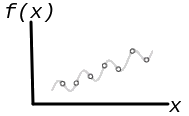
\includegraphics[scale=0.8]{figs/grafA.png}
        \label{fig:graf1:grafA} }
    \quad
    \subfloat[Função \textbf{h} com hipótese linear]{
        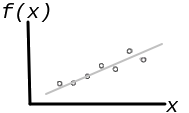
\includegraphics[scale=0.8]{figs/grafB.png}
        \label{fig:graf1:grafB} }
    
    \caption{Hipóteses ajustadas – Função ${h}$ próxima da função ${f}$ real} \label{fig:graf1}
        
        %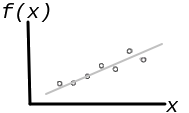
\includegraphics[scale=0.4]{figs/grafB.png}
        %\caption{Polinômio Superajustado} \label{grafB}
\end{figure}


O exemplo da figura \ref{fig:graf1:grafA} mostra a função ${h}$  de grau 6,na qual acontece um sobreajuste (\textit{overfitting}) no conjunto de dados de treinamento. Esse modelo exibe uma função mais complexa para atendera todo o conjunto de dados do gráfico, tornando-se um modelo específico para essa amostra de dados. 

Já na figura \ref{fig:graf1:grafB}, o ajuste da função ${h}$ se torna mais simples e mesmo o gráfico não passando por todos os pontos, acabou por generalizar melhor o conjunto de treinamento, tornando, um melhor resultado da predição de novos valores. 

Em análise da figura \ref{fig:graf1} são apresentadas duas hipóteses que tentam se aproximar ao máximo da função verdadeira (${f}$), que é desconhecida. Mesmo parecendo que na figura \ref{fig:graf1:grafA} obteve-se melhor resultado, pois todos os pontos são atingidos pelo gráfico da função, este modelo acabou se ajustando muito bem na amostra de dados, deixando a função ${h}$ muito específica, não retratando os dados em um mundo real. Então, apesar de parecer que a figura \ref{fig:graf1:grafA} é  a melhor opção por ela ser mais específica, não é, pois quanto mais generalizado for o modelo, melhor será para predizer os valores de ${y}$ para novos conjuntos de dados.

O treinamento dos dados realizado nesta pesquisa utilizou validação cruzada com o número  ${k}$ igual a dez  para os três algoritmos. Este ${k}$ indica que o algoritmo supervisionado irá treinar com os dados dividido em dez subgrupos, onde um subgrupo é utilizado para validar os teste dos outros subgrupos restantes. Esse procedimento é feito ${k}$ vezes alternando mutuamente entre os subgrupos e retirado uma média que é o valor resposta do algoritmo aplicado.


\subsubsection{Algoritmo Classification And Regression Trees  - CART}\label{cap:refTeor:sssec:cart}


O algoritmo Classification And Regression Trees - CART constrói modelos de previsão a partir de dados de treinamento e seus resultados podem ser representados em uma árvore de decisão. Esta árvore  é uma ferramenta que dá suporte a uma escolha utilizando como modelo um fluxograma semelhante a uma árvore, em que, a cada nó interno, é feito um teste, tendo como resposta “sim” ou “não” (a exemplo da figura \ref{fig:fluxogramaarvore}), permitindo uma abordagem do problema de forma estruturada e sistemática até chegar a uma conclusão lógica. ``Uma árvore de decisão alcança sua decisão executando uma sequência de testes'' \cite[p. 811]{RusselStuart.Norvig2013}

 \begin{figure}[h!]
    \centering
      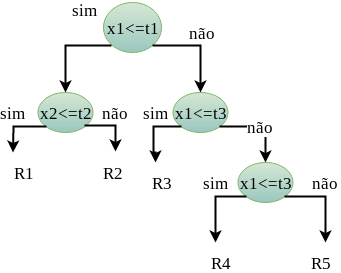
\includegraphics[scale=0.5]{figs/arvoredecisao_nos.png}
      \caption{Exemplo de Fluxograma de árvore: R1 a R5 são as folhas relacionadas de acordo com as respostas sim ou não dos nós} \label{fig:fluxogramaarvore}
\end{figure}

O CART pode se tornar uma árvore de classificação ou também uma árvore de regressão. O que definirá o tipo de árvore é o valor do atributo “classe”, se categórico ou contínuo. Por exemplo, em um conjunto de dados de um paciente que tenta prever se  ele possuirá câncer, ou não, a classe seria ``Terá Câncer'' ou ``Não terá Câncer'', podendo esse atributo assumir duas categorias (classes) e assumindo uma árvore de classificação. Na regressão, o atributo ``classe'' pode assumir um valor contínuo, tornando-se uma árvore de regressão, que poderá prever valores numéricos como: período de tempo de internação do paciente, preço de uma cirurgia, temperatura do paciente ou quantidade de água ingerida. No caso de não ser probabilístico, o grau de confiança em seu modelo de predição será embasado em respostas semelhantes em outras circunstâncias antes analisadas e utiliza uma técnica como partição recursiva binária, na qual cada nó pai é sempre decomposto em dois nós filhos, e cada nó filho irá ser tratado posteriormente no processo como nó pai. 

De acordo com \citeonline{yohannes1999classification,Raimundo2008}, existem três componentes importantes na construção de uma árvore de decisão:
%Na construção de uma árvore de decisão existem três componentes importantes de acordo com \citeonline{yohannes1999classification,Raimundo2008}: 
%Para construção de uma árvore, pode-se simplificar em três componentes importantes \cite{yohannes1999classification,Raimundo2008}: 

\begin{itemize}
[noitemsep]
 \item Um conjunto de perguntas que servirá de base para fazer uma divisão de um nó;
 \item Regras de divisão para julgar o quanto é boa esta divisão;
 \item Regras para atribuir uma classe a cada nó;
\end{itemize}

Na divisão inicial será atribuída ao nó pai uma questão e,  dependendo da resposta (sim ou não - a exemplo da figura \ref{fig:fluxogramaarvore}), os registros irão para nó filho esquerdo ou direito, e depois será realizado o teste do ponto de divisão. O CART percorrerá todos os atributos e construirá uma árvore de decisão baseada no melhor ponto de divisão, uma vez que são testados todos os atributos como potencial divisor. Após a escolha do melhor ponto de divisão do nó, faz-se a atribuição de uma classe para o nó e, após essa etapa, o novo nó filho passa a ser nó pai, refazendo os mesmos passos anteriores para sua divisão.

A equação \ref{eq:cartGini} é utlizado pelo CART para escolher a divisão dos nós em função da regra Gini de Impureza \cite{breiman1984}. É definido o grau de pureza variando de 0 (zero) a 1 (um), portanto, quando o nó tende a um resultado de índice Gini aproximando-se de 1 (um), maior a impureza do nó, e o inverso, maior a pureza. A equação \ref{eq:cartGini} mede a impureza do conjunto ${S}$ e caso todos os dados forem da mesma classe (dados puros), o resultado da equação seria ${1-1=0}$.

\begin{equation}
Gini(S)= 1 - \sum [p(j/t)]^2
 \label{eq:cartGini}
\end{equation}
Onde: ${p(j/t)}$ é probabilidade a \textit{priori} da classe ${j}$ se formar no nó ${t}$, e ${S}$ é um conjunto de dados que contém exemplos de n classes.
%\begin{itemize}
% \item ${S}$: é um conjunto de dados que contém exemplos de n classes
% \item ${p_j}$: é uma frequência relativa da classe ${j}$ em ${S}$
%\end{itemize}
 

Este cálculo tem como finalidade a escolha da divisão do nó (conjunto ${S}$), em que é medida a impureza da divisão do nó pai com os nós filhos, e para isso, contém a média ponderada de cada índice do subgrupo formado por essa divisão de ${S}$. Então o menor valor encontrado em ${Gini_{split}(S)}$ será o escolhido para dividir o nó, de acordo com a equação \ref{eq:cartGiniSplit}.

\begin{equation}
Gini_{split}(S) = \frac{S_l}{S}gini(S_l)+\frac{S_r}{S}gini(S_r)
 \label{eq:cartGiniSplit}
\end{equation}
Onde:
\begin{itemize}[noitemsep]
            \item ${S}$ conjunto de dados que contém exemplos de n classes;
            \item ${S_l}$ subconjunto esquerdo de ${S}$;
            \item ${S_r}$ subconjunto direito de ${S}$;
        \end{itemize}

Para a escolha da variável e ponto de divisão necessário do nó, terão que ser aplicados testes em todos os atributos através das equações \ref{eq:cartGini} e \ref{eq:cartGiniSplit} e após o envolvimento de todos os atributos, será escolhido o nó com menor valor ${Gini_{split}(S)}$.


%só assim é possível saber qual melhor ponto de divisão. Caso o valor do atributo seja contínuo será necessário ordenar os registros do atributo e encontrar os pontos médios entre os valores sucessivos. Ex.

%No procedimento da divisão do nó em dois subconjuntos, o atributo poderá conter valores contínuos ou categóricos. Quando o atributo possuir valores contínuos - por exemplo, ${[4.2, 2.0, 1.0, 8.8,...,10.8]}$, estes serão ordenados ${[1.0, 2.0, 4.2, 8.8,...,10.8]}$, e após, serão encontrados valores entre os pontos (por exemplo o ${1.5}$ que está entre ${1.0}$ e ${2.0}$), e assim sucessivamente até o último dois pontos. Para cada valor  encontrado os registros serão divididos: menor igual (<=) a ${1.5}$ e maior (>) ${1.5}$. No seguinte caso serão aplicados a equação \ref{eq:cartGiniSplit} em todos os números encontrados, e escolhido o menor valor para saber o melhor ponto de divisão. Em outra situação, sendo as variáveis  categóricas - por exemplo X, Y e Z, terão que ser testadas qual melhor divisão entre elas: \{X\} e \{Y,Z\}, \{Y\} e \{X,Z\} ou \{Z\} e \{X,Y\}. 

No procedimento da divisão do nó em dois subconjuntos, o atributo poderá conter valores contínuos ou categóricos. Nas duas opções será aplicada a equação \ref{eq:cartGiniSplit} em todos os valores e escolhido o melhor ponto de divisão. No caso de serem valores contínuos, simplesmente após o valor ser o escolhido para a divisão, ela será menor, igual (ramo da esquerda) ou maior (ramo da direita) que o valor escolhido. Em outra situação, sendo as variáveis categóricas - por exemplo X, Y e Z, terá que ser testada, dentre todas as possibilidades, qual a melhor divisão entre elas e como é uma divisão binária, pois o nó não poderá ser dividido em 3 (três) ramos X, Y e Z, e sim em grupos de dois, como:\{X\} e \{Y,Z\}, \{Y\} e \{X,Z\} ou \{Z\} e \{X,Y\}.

%No procedimento da divisão do nó em dois subconjuntos, o atributo poderá conter valores contínuos ou categóricos. Nas duas opções serão aplicados a equação \ref{eq:cartGiniSplit} em todos os valores, e escolhido o melhor ponto de divisão. No caso de serem valores contínuos, simplesmente após o valor ser o escolhido para a divisão, esta divisão será: menor igual (ramo da esquerda) ou maior (ramo da direita) que o valor escolhido. Em outra situação, sendo as variáveis  categóricas - por exemplo X, Y e Z, terão que ser testadas, dentre todas as possibilidades, qual melhor divisão entre elas, e como é uma divisão binária, o nó não poderá ser dividido em 3 (três) ramos X, Y e Z, e sim, em grupos de dois como: \{X\} e \{Y,Z\}, \{Y\} e \{X,Z\} ou \{Z\} e \{X,Y\}.

% De acordo com \citeonline{yohannes1999classification,Raimundo2008}, existem três componentes importantes na construção de uma árvore de decisão:
% %Na construção de uma árvore de decisão existem três componentes importantes de acordo com \citeonline{yohannes1999classification,Raimundo2008}: 
% %Para construção de uma árvore, pode-se simplificar em três componentes importantes \cite{yohannes1999classification,Raimundo2008}: 
% 
% \begin{itemize}
% [noitemsep]
%  \item Um conjunto de perguntas que servirá de base para fazer uma divisão;
%  \item Regras de divisão para julgar o quanto é boa esta divisão;
%  \item Regras para atribuir uma classe a cada nó;
% \end{itemize}
% 
% Na divisão inicial será atribuído ao nó pai uma questão onde dependendo da resposta (sim ou não) os registros irão para nó filho esquerdo ou direito, e após, será realizado o teste do ponto de divisão. O CART percorrerá todos os atributos e construirá uma árvore de decisão baseado no melhor ponto de divisão, uma vez que são testados todos os atributos como potencial divisor, e escolhido o que tiver maior índice Gini. Após a escolha do melhor ponto de divisão do nó faz-se a atribuição de uma classe para o nó, e após essa etapa, o novo nó filho passa a ser nó pai, refazendo os mesmos passos anteriores para a divisão desse nó.






% 
% \IncMargin{1em}
% \begin{algorithm}[h!]
% 
% \nl $melhorGini$; \tcc{cria a variável}
% \nl $divisaoCorrente \leftarrow 4.9$;\tcc{Ex. recebe o 1º valor do atributo} 
% \nl $direita \leftarrow 0$\; 
% \nl $esquerda \leftarrow 6$;\tcc{Ex. recebe o total de dados existentes para o atributo} 
% \nl \While{existirem dados}{
%  \nl \If{1ª Dado Lista do Atributo MAIOR $divisaoCorrente$}{ 
%       \nl $valorGini \leftarrow calculaGini(divisaoCorrente)$; 
%       } 
%  \nl \Else{ 
%         \nl$valorGini \leftarrow calculaGini(1ªDadoLista)$;
%         }
%  \BlankLine
%  
%  \nl \If{ Primeiro Gini encontrado}{
%         \nl $melhorGini \leftarrow valorGini$;
%         }
%     \nl \Else{
%         \nl \If{$valorGini > melhorGini$}{
%                 \nl $melhorGini \leftarrow valorGini$
%                 }
%             }        
%   \nl $divisaoCorrente \leftarrow 5.4$; \tcc{recebe o próximo dado do atributo}
%   \nl $direita$ recebe o que possui +1 e $esqueda$ o -1\;
%   \nl $(valorGini + divisaoCorrente)/2$;\tcc{encontrar ponto de divisão}
%  }
%  \caption{Rotina de funcionamento do CART com critério Gini \cite{Raimundo2008} }\label{alg:gini}
%  
% \end{algorithm}
% \DecMargin{1em}


\subsubsection{Algoritmo Naive Bayes}\label{cap:refTeor:sssec:nbayes}

O algoritmo bayesiano Naive Bayes é um modelo probabilístico de aprendizado que pode ser calculado diretamente entre seus dados de treinamento. Depois de calculado, o modelo pode ser utilizado para fazer previsões de novos dados através do teorema de Bayes. ``O teorema de Bayes fornece uma maneira de calcular a probabilidade de uma hipótese com base em sua probabilidade anterior, as probabilidades de observar vários dados, dadas as hipóteses, e os dados observados em si'' \cite[p. 156]{Mitchell1997}.



Esse teorema utiliza uma teoria estatística e probabilística para previsão de acontecimento de um evento, sendo este evento relacionado à condição da probabilidade de ocorrências anteriores a ele, portanto, é nesse segmento que o algoritmo Naive Bayes funciona, criando classificadores probabilísticos baseados no teorema de Bayes. 


Pode-se citar, como exemplo desse evento, a descoberta do câncer em uma pessoa, pois se tal doença estiver relacionada ao sexo, então, utilizando o teorema de Bayes, o sexo de uma pessoa pode ser utilizado para dar maior precisão à probabilidade de câncer, em vez de fazer uma avaliação de probabilidade sem a utilização dele.

O Naive Bayes utiliza uma técnica de independência dos atributos, em que cada variável de entrada não depende de recursos de outras. Essa independência condicionada, entre os atributos que nem sempre ocorrem nos problemas reais, acabou ficando conhecida por Bayes ingênuo ou Naive Bayes. 

Em \citeonline{RusselStuart.Norvig2013} a equação \ref{eq:causaefeito} mostra a relação ${P(causa/efeito)}$ onde o efeito é evidência de alguma causa desconhecida, e quer se determinar a causa. Logo em seguida as equações \ref{eq:bayes} e \ref{eq:bayes:numerador} são responsáveis pelo cálculo de probabilidade do algoritmo.

\begin{equation} \label{eq:causaefeito}
 P(causa|efeito)= \frac{P(efeito|causa)P(causa)}{P(efeito)}
\end{equation}

Naive Bayes como classificador estatístico possui um modelo de simples construção, e ficou conhecido por ter bons resultados em relação a algoritmos mais sofisticados, mesmo trabalhando com grandes quantidades de dados, e possui uma característica de agrupar objetos de uma certa classe em razão da probabilidade do objeto pertencer a esta classe. 

\begin{equation}
 P(c/x)= \frac{P(x/c)P(c)}{P(x)}
\label{eq:bayes}
 \end{equation}

\begin{equation}
 P(x/c)=P(x_1|c)*P(x_2|c)*...*P(x_n|c)*P(c)
 \label{eq:bayes:numerador}
\end{equation}


\begin{itemize}[noitemsep]
 \item ${P(c/x)}$ probabilidade posterior da classe ${c,alvo}$ dada preditor ${x,atributos}$.
 \item ${P(c)}$  é a probabilidade original da classe.
 \item ${P(x|c)}$  é a probabilidade que representa a probabilidade de preditor dada a classe.
 \item ${P(x)}$  é a probabilidade original do preditor.
\end{itemize}

A utilização do algoritmo Naive Bayes já é bem difundida e está presente em vários trabalhos, como classificação de textos, filtro de SPAM, analisador de sentimentos, entre outros \cite{Madureira2017, Lucca2013, Wu2008, Mccallum1997}, entretanto, mesmo atingido boa popularidade, o algoritmo se utiliza da suposição de ter preditores independentes e isso não acontece muito na vida real, pois acaba sendo difícil ter uma amostra de dados que sejam inteiramente independentes. 

\begin{table}[!ht]
\centering
%\resizebox{\textwidth}{!}{ 
\begin{tabular}{|l|l|l|l|l|l|}
\hline \hline 
\rowcolor[HTML]{EFEFEF} 
     & Aspecto   & Temperatura  & Umidade   & Vento    & Decisão \\ \hline
1       & Sol       & Quente        & Alta   & Fraco       & Não \\ \hline                    
2       & Sol       & Quente        & Alta   & Forte       & Não \\ \hline
3       & Nublado   & Quente        & Alta   & Fraco       & Sim \\ \hline                    
4       & Chuva     & Agradável     & Alta   & Fraco       & Sim \\ \hline
5       & Chuva     & Fria          & Normal   & Fraco       & Sim \\ \hline                    
6       & Chuva     & Fria          & Normal   & Forte       & Não \\ \hline
7       & Nublado   & Fria          & Normal   & Forte       & Sim \\ \hline                    
8       & Sol       & Agradável     & Alta   & Fraco       & Não \\ \hline
9       & Sol       & Fria          & Normal   & Fraco       & Sim \\ \hline                    
10       & Chuva    & Agradável     & Normal   & Fraco       & Sim \\ \hline
11       & Sol      & Agradável     & Normal   & Forte       & Sim \\ \hline                    
12       & Nublado  & Agradável     & Alta   & Forte       & Sim \\ \hline
13       & Nublado  & Quente        & Alta   & Fraco       & Sim \\ \hline                    
14       & Chuva    & Agradável     & Alta   & Forte       & Não \\ \hline
\end{tabular}
%}
\caption{Base de exemplo onde exibe através do atributo Decisão, se existe, ou não condição de jogo perante as outras características (Aspecto, temperatura, Umidade e Vento)}
\label{tab:exemploNB}
\end{table}

A tabela \ref{tab:exemploNB} é uma amostra de dados, na qual é possível aplicar o funcionamento do Naive Bayes através da equação \ref{eq:bayes}, sendo esta tabela composta por 4 (quatro) características (Aspecto, Temperatura, Umidade e Vento) e pela coluna Decisão, representando a classe. 

Então, cada registro assume uma condição de jogo ´´Sim'' ou ``Não'' - por exemplo, na linha 2 (dois) faz ``Sol'', é ``Quente'', possui umidade ``Alta'' e vento ``Forte'' e existe no atributo classe a não possibilidade de jogo (Decisão = Não). Pode-se com as informações dessa amostra prever algumas possibilidades de jogo, dependendo de como estão dispostos os valores dessas características. Para exemplificar melhor, as seguintes condições são para saber se há possibilidade de jogo, ``Sim'': P(Jogar=sim|Aspecto=sol, Temperatura=fria, Umidade=alta e Vento=forte). Para obter a resposta, será necessária a aplicação na equação \ref{eq:bayes}.

 


\begin{eqnarray}
&=& \frac{ P(Sol|Sim)*P(Fria|Sim)*P(Alta|Sim)*P(Forte|Sim)*P(Sim) }{ P(Sol)*P(Fria)*P(Alta)*P(Forte) } \nonumber \\ \\
 &=& \frac{ \frac{2}{9}*\frac{3}{9}*\frac{3}{9}*\frac{3}{9}*\frac{9}{14} }{ \frac{5}{14}*\frac{4}{14}*\frac{7}{14}*\frac{6}{14} } \nonumber \\ \\
 &=& \frac{0,0053}{0,02186} \nonumber \\ \\
 &=& 0,242
 \label{eq:resolNB}
\end{eqnarray}

O resultado (${0,242}$) mostra uma probabilidade aproximada de ${20\%}$ de chance de acontecer o jogo de acordo com as características apresentadas, implicando aproxima- damente ${80\%}$ de não acontecer, portanto, seguindo esse resultado, pode-se afirmar que a previsão é de não ocorrer o jogo. 


\subsubsection{Algoritmo k-Nearest Neighbor - KNN}\label{cap:refTeor:sssec:knn}

O K-Nearest Neighbor - KNN é um algoritmo de classificação simples, em que os objetos são classificados por meio de um conjunto de treinamento que estão próximos no espaço de características. Uma vez que seja necessário definir qual a classificação de um objeto, serão averiguados quais são os exemplos mais próximos determinados por uma distância e assim se definirá, por meio desses elementos próximos, qual sua classificação. 

Na execução do KNN algumas considerações são importantes, como a definição da métrica entre os elementos e o número que a variável K assumirá; ademais, seguem alguns passos: i) o algoritmo funcionará calculando a distância entre todos os exemplos próximos do elemento a classificar; ii) serão identificados os K vizinhos mais próximos; iii) e através do número de K será determinada a mesma classe do vizinho para classificação do elemento. 

Na figura \ref{fig:knn} pode-se observar o comportamento do algoritmo:  um objeto está próximo de outros objetos vizinhos e o número de vizinhos é determinado pelo K.

\begin{figure}[h!]
    \centering
    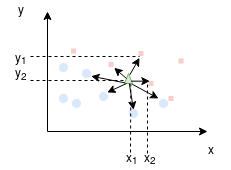
\includegraphics[scale=0.9]{figs/ex_knn1.png}
    
    
    \caption{Exemplo do funcionamento do algoritmo KNN} 
    \label{fig:knn}     
        %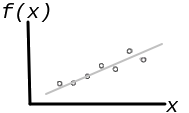
\includegraphics[scale=0.4]{figs/grafB.png}
        %\caption{Polinômio Superajustado} \label{grafB}
\end{figure}

Neste exemplo da figura \ref{fig:knn} um novo objeto precisa ser classificado e na amostra de dados distribuída no plano cartesiano o algoritmo KNN prevê sua classificação de acordo com objetos que estão próximos a ele. Na figura \ref{fig:knn} existem objetos ``círculos'', ``quadrados'', e um novo objeto ``triângulo'' a ser classificado. 

O algoritmo KNN calcula a distância do objeto ``triângulo'' para com os outros objetos utilizando a distância euclidiana \cite{Lachi2005}, conforme equação \ref{eq:euclidiana} que está na forma bidimensional de acordo com o exemplo apresentado na figura \ref{fig:knn}.

\begin{equation}
d=\sqrt{(x_2-x_1)^2 + (y_2-y_1)^2}
 \label{eq:euclidiana}
\end{equation}

Onde:
\begin{itemize}[noitemsep]
 \item ${d}$ resultado da distância euclidiana entre dois objeto no plano cartesiano;
 \item ${x_2-x_1}$ distância no eixo ${x}$ entre objetos;% nas coordenadas ${x_2}$ e ${x_1}$;  
 \item ${y_2-y_1}$ distância no eixo ${y}$ entre  objetos;% nas coordenadas ${y_2}$ e ${y_1}$;  
\end{itemize}

Ao calcular todas as distâncias, o algoritmo irá ordenar estes resultados de forma crescente de acordo com a tabela \ref{tab:exemploKNN} e depois, dependendo do valor de ${K}$, será determinada a classe do objeto. A tabela de exemplo é formada por 3 (três) colunas, em que ${K}$  significa o número de vizinhos, seguida da distância e também qual o tipo de objeto (quadrado ou círculo). 



\begin{table}[!ht]
\centering 
\begin{tabular}{|c|c|c|}
\hline \hline 
\rowcolor[HTML]{EFEFEF} 
K & Distância     & Classe \\ \hline
1 & 0,11       & 
\includegraphics[scale=0.2]{figs/circulo.png}       \\ \hline                    
2 & 0,29       &  
\includegraphics[scale=0.2]{figs/quadrado.png}        \\ \hline
3 & 1,10       &  
\includegraphics[scale=0.2]{figs/quadrado.png}   \\ \hline                    
4 & 1,40       &  
\includegraphics[scale=0.2]{figs/circulo.png}     \\ \hline
5 & 1,55       &  
\includegraphics[scale=0.2]{figs/circulo.png}     \\ \hline                    
\end{tabular}
%}
\caption{Tabela em ordem crescente das distâncias euclidianas encontradas do objeto a que se deseja classificar para os outros objetos da amostra, de acordo com as setas da figura \ref{fig:knn}}
\label{tab:exemploKNN}
\end{table}


 
Para definir qual a classe que o objeto ``triangulo'' assumirá, será necessário saber qual valor de ${K}$, pois o maior número de ocorrências de uma determinada classe será a classe eleita para o novo objeto - por exemplo, utilizando a tabela \ref{tab:exemploKNN}, com ${K=1}$, a classe deste registro é “círculo”, dado que o número de ocorrências é CÍRCULO=1 e QUADRADO=0, então, caso ${K=1}$, o número de ocorrência do “círculo” é maior que ``quadrado''. 

No caso de ${K=2}$, aparece uma ocorrência de “círculo” e uma ocorrência de “quadrado”, totalizando CÍRCULO=1 e QUADRADO=1; nesse caso, não fica definida qual a classe, pois cada uma possui o mesmo número de ocorrências. 

Já com ${K=3}$, a contagem de ocorrências em cada classe totaliza CÍRCULO=1 e QUADRADO=2 e, desta vez, a classe que possui maior número de ocorrências é a escolhida para o novo objeto ``quadrado'' e assim acontece sucessivamente para os outros valores ${K}$ assumirem. Cada vez que o valor de ${K}$ aumenta é feita a soma de ocorrências de cada classe, sendo a classe eleita a que apresentar mais ocorrências. 
 

Ao escolher um valor par de ${K}$, poderá haver um empate no número de ocorrências das classes. Essa situação fica clara no exemplo acima, tabela \ref{tab:exemploKNN}, quando ${K=2}$  (CÍRCULO=1 e QUADRADO=1) e ${K=4}$  (CÍRCULO=2 e QUADRADO=2); para não acontecer um valor de empate, é necessário escolher sempre um valor ${K}$ ímpar e este parâmetro é definido ao executar o algoritmo. 

Diferente do estudo de  \citeonline{Lopes2016} que em determinada fase de seu trabalho testou um algoritmo de paradigma conexionista para fazer rotulação, esta pesquisa aplicou algoritmos com paradigmas diferentes: bayesiano, simbolista e analogista  \citeonline{pedro2017}, comprovando que também é possível realizar rotulação de dados.

% Os três algoritmos de aprendizado supervisionados acima mencionados foram aplicados nas  bases de dados para fazer rotulação. \citeonline{Lopes2016}, testou somente um algoritmo de paradigma conexionista, nesta pesquisa outros algoritmos com paradigmas diferentes foram testados: bayesiano, simbolista e analogista (baseado em instâncias), conforme autor \citeonline{pedro2017} cita em sua obra. 

O primeiro, Naive Bayes, um algoritmo probabilístico bayesiano, possue uma característica de destaque, que é, a não dependência entre atributos em seus cálculos. O CART, outro algoritmo, é um exemplo simbolista implementado em árvore de decisão, e KNN, paradigma baseado em instâncias, que faz classificação levando em consideração a distâncias entre os espaço de características, mas possui melhores resultados quando aplicado em bases de pouca dimensionalidade - \textit{i.e.}, quanto mais características menor a performance do modelo.

\subsection{Aprendizado Não-Supervisionado}\label{ssec:aprendNSup}

Outro modelo de aprendizado de máquina é o aprendizado não-supervisionado, em que não existe uma tentativa de se encontrar uma função que se aproxime da real, logo porque os registros não são classificados, visto que o conjunto de treinamento não possui informação da saída sobre determinada entrada. Desta forma, os algoritmos procuram algum grau de similaridade entre os registros e tentam agrupá-los de forma a ter algum sentido para estarem juntos.

Quando o algoritmo encontra dados com mesma similaridade a ele, estes são agrupados, formando \textit{clusters}. Os números de \textit{clusters} encontrados dependerá do funcionamento, técnica, configuração dos algoritmos e também do grau de dissimilaridade entre elementos de grupos diferentes. Segundo \citeonline{Barber2011} não existe uma variável “classe” no aprendizado não-supervisionado, então, o maior interesse seria em uma perspectiva probabilística de distribuição p(x) de um determinado conjunto de dados ${D = \{x_{n},n=1,...,N\}}$. Mesmo não possuindo rótulos (classes), novos dados inseridos são submetidos aos algoritmos não-supervisionados e esses algoritmos são capazes de encontrar padrões nos atributos em um conjunto de treinamento, conseguindo inferir sobre os dados de testes, classificando-os em algum grupo.

Cada algoritmo utilizará alguma característica para determinar grupos diferentes na base de dados; no exemplo da figura \ref{fig:planoCartesianoAprendNSup}, fica visível por conta dos círculos coloridos a existência de agrupamentos diferentes (h1, h2, h3, h4). 

\begin{figure}[h!]
    \centering
    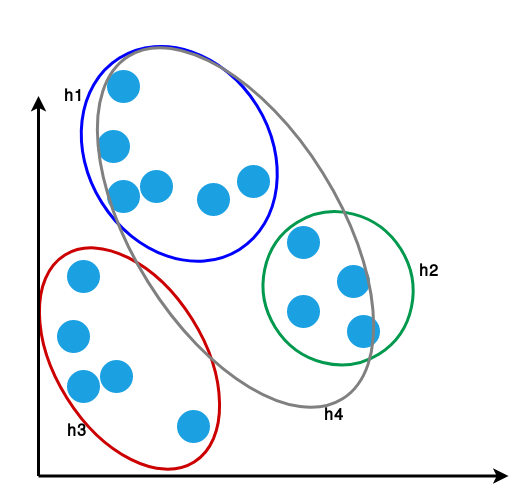
\includegraphics[scale=0.4]{figs/amostra_dados_AprendNSuperv.png}
    
    
    \caption{Exemplos de técnicas diferentes utilizada por algoritmos para dividir em grupos} 
    \label{fig:planoCartesianoAprendNSup}     
        %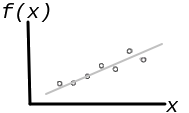
\includegraphics[scale=0.4]{figs/grafB.png}
        %\caption{Polinômio Superajustado} \label{grafB}
\end{figure}

% \begin{equation}
%  D = \{x_{n},n=1,...,N\}
%  \label{eq:aprendNSup}
% \end{equation}

 

O que é apresentado na figura \ref{fig:planoCartesianoAprendNSup} são situações de agrupamentos em um conjunto distribuído bidimensional. Dependendo do algoritmo, ou mesmo da configuração, é possível ter 3 (três) grupos formados por h1, h2 e h3, ou 2 (dois) grupos formados por h3 e h4, ou mesmo, um grupo só pela união de h3 e h4. 

\section{Discretização}\label{cap:refTeor:sec:discret}

O método de discretização faz a conversão de valores contínuos em valores discretos. A partir de um atributo com valores contínuos, a discretização cria um ponto inicial e final definindo um intervalo e designando uma faixa para cada intervalo. Assim, ao invés de valores contínuos, teremos valores discretos representando as faixas de valores. 

Segundo alguns autores, a discretização melhora a precisão e deixa um modelo de classificador mais rápido em seu conjunto de treinamento \cite{Catlett2006b,Hwang2002}. De acordo com \cite{Kotsiantis2006, Dougherty1995}, os métodos de discretização mais comumente utilizados, no âmbito dos métodos não-supervisionados, são os de Discretização por Larguras Iguais (do inglês: Equal Width Discretization - EWD) e Discretização por Frequências Iguais (do inglês: Equal Frequency Discretization - EFD). Em quanto de um lado a discretização ajuda no treinamento do modelo, por outro, ambos os métodos sofrem com perda de informação, pois o número de faixas designado não é determinado levando em consideração as propriedades dos dados de treinamento, e dependendo do número de faixas há uma menor ou maior perda. 

Mesmo com uma consequente perda, a discretização tem um papel importante na rotulação e dependendo dos tipos de dados, método e das faixas, os rótulos sofrerão alterações, \textit{e.g.}, pode haver registros que estejam representados em uma determinada faixa, ao alterar o método de discretização também altera o corte da faixa, fazendo esse registro mudar de faixa, consequentemente o rótulo também muda, gerando uma nova visão ao analista do \textit{cluster}. 


%Aqui nesse trabalho é utilizado a técnica de discretização antes da execução dos algoritmos e as faixas selecionadas são usadas para identificar o rótulo. Após o conhecimento do rótulo o valor da faixa é trocado pelo início e fim do intervalo.



\subsection{Equal Weight Discretization - EWD}\label{cap:refTeor:subsec:ewd}

O método de Discretização por Larguras Iguais (Equal Weight Discretization - EWD) faz a discretização de um intervalo, entre valores contínuos, dividindo através de um ponto de corte as faixas de tamanhos iguais \cite{Baron2016,Yang2002}. Logo, se existir um intervalo com valores contínuos [a,b] e deseja particionar em ${R}$ faixas de tamanhos iguais, serão necessários ${R-1}$ pontos de corte. Na figura \ref{fig:pontocorte} exibe exatamente o que foi dito, caso tenha um ${R=2}$ simulando duas faixas em um intervalo ${[a,b]}$.


\begin{figure}[h]
        \centering
        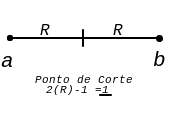
\includegraphics[scale=1]{figs/faixaA-B_PontoCorte.png}
        \caption{Ponto de Corte (R-1); 2(R) significa o valor de R=2; 2 - 1 = 1} \label{fig:pontocorte}
\end{figure}

Para exemplificar, a figura \ref{fig:pontocorte} exibe uma faixa com início em ``[a'', e final ``b]'', e pretende obter a divisão do intervalo ${[a,b]}$ em 2 (duas) faixas iguais (${R=2}$), então, utilizando a regra ( Número\_De\_Faixas - 1 =  2-1=1), obtendo sempre o número de faixas que deseja particionar, menos 1 (um).

Para haver o ponto de corte, terá que ser feita primeiro a ordenação dos dados e logo após definir a largura de cada faixa ${r_1,...,r_R}$. O cálculo realizado na equação \ref{eq:largurafaixa}, para encontrar ${w}$, é a diferença entre os limites superior e inferior do intervalo, dividido pela quantidade de faixas (${R}$).

\begin{equation}
 w = \frac{b-a}{R}
 \label{eq:largurafaixa}
\end{equation}
\begin{itemize}[noitemsep]
 \item ${w}$ - tamanho da faixa
 \item a,b - limite inferior, limete superior respectivamente
 \item R - número de faixas
\end{itemize}

De acordo com a figura \ref{eq:regratamfaixa}, a variável ${w}$ delimita o tamanho das faixas de valores e determina os pontos de corte ${(c_1,...,c_{R-1})}$. O primeiro ponto de corte, ${c_1}$, é obtido por meio da soma do limite inferior ${a}$ com a tamanho de ${w}$, e os pontos de corte seguintes são calculados pela soma do ponto de corte anterior com ${w}$.

\begin{equation}
c_i=\left\{\begin{matrix}
a+w, & se\, i=1 & \\ 
c_{i-1}+w,  & caso\, contrário & 
\end{matrix}\right.
 \label{eq:regratamfaixa}
\end{equation}
\begin{itemize}[noitemsep]
 \item ${w}$ - tamanho da faixa
 \item ${c_i}$ - ponto de corte da faixa
 \item a - limite inferior
\end{itemize}

Seguindo a figura \ref{fig:faixasEWD}, o valor da faixa do intervalo ${[a,c_1]}$ será o valor discreto igual ao índice de sua faixa, nesse caso ${r_1}$, então, o valor na faixa ${r_1}$ é reprensentado por ${1(um)}$, pois  ${i=1}$. No caso do intervalo ${]c_1,c_2]}$ definido na faixa  ${r_2}$, é representado pelo valor discreto 2 (dois) e, e consequentemente, o valor que se encontra em uma faixa qualquer ${r_i}$ será reprensentado por ${i}$.

%\afterpage{
\begin{figure}[h] 
        \centering
        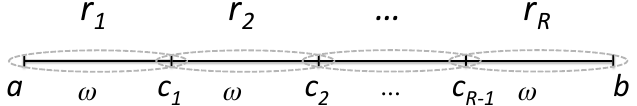
\includegraphics[scale=0.6]{figs/discretizacaoEWD.png}
        \caption[Discretização EWD]{Discretização EWD. Figura baseada em \cite{Lopes2016}}%\footnotemark } 
        \label{fig:faixasEWD}
\end{figure}
%\footnotetext{Figura extraída de \cite{Lopes}}
% }

A tabela \ref{tab:amostraDiscret} contém uma amostra de valores dividida em duas colunas: a primeira coluna significa o número da linha e a segunda coluna o valor propriamente dito. Essa tabela servirá para exemplificar o que foi dito neste método de discretização e pode ser vista como um vetor de 150 (cento e cinquenta) posições e, dependendo do número de faixas, poderá ser dividido em vários pedaços, sendo cada pedaço uma faixa. 

\begin{table}[!ht]
\centering

\begin{tabular}{|l|l|}
\hline 
 no. & Valor \\ \hline
1	&	5.10	\\ \hline
2	&	4.90	\\ \hline
3	&	4.70	\\ \hline
4	&	4.60	\\ \hline
5	&	5.00	\\ \hline
6	&	5.40	\\ \hline
7	&	4.60	\\ \hline
8	&	5.00	\\ \hline
9	&	4.40	\\ \hline
10	&	4.90	\\ \hline
11	&	5.40	\\ \hline
12	&	4.80	\\ \hline
13	&	4.80	\\ \hline
14	&	4.30	\\ \hline
15	&	5.80	\\ \hline
16	&	5.70	\\ \hline
17	&	5.40	\\ \hline
18	&	5.10	\\ \hline
19	&	5.70	\\ \hline
20	&	5.10	\\ \hline
21	&	5.40	\\ \hline
22	&	5.10	\\ \hline
23	&	4.60	\\ \hline
24	&	5.10	\\ \hline
25	&	4.80	\\ \hline
\end{tabular}
\begin{tabular}{ |l|l| }
\hline
 no. & Valor \\ \hline
26	&	5.00	\\ \hline
27	&	5.00	\\ \hline
28	&	5.20	\\ \hline
29	&	5.20	\\ \hline
30	&	4.70	\\ \hline
31	&	4.80	\\ \hline
32	&	5.40	\\ \hline
33	&	5.20	\\ \hline
34	&	5.50	\\ \hline
35	&	4.90	\\ \hline
36	&	5.00	\\ \hline
37	&	5.50	\\ \hline
38	&	4.90	\\ \hline
39	&	4.40	\\ \hline
40	&	5.10	\\ \hline
41	&	5.00	\\ \hline
42	&	4.50	\\ \hline
43	&	4.40	\\ \hline
44	&	5.00	\\ \hline
45	&	5.10	\\ \hline
46	&	4.80	\\ \hline
47	&	5.10	\\ \hline
48	&	4.60	\\ \hline
49	&	5.30	\\ \hline
50	&	5.00	\\ \hline
\end{tabular}
\begin{tabular}{ |l|l| }
\hline
 no. & Valor \\ \hline
51	&	7.00	\\ \hline
52	&	6.40	\\ \hline
53	&	6.90	\\ \hline
54	&	5.50	\\ \hline
55	&	6.50	\\ \hline
56	&	5.70	\\ \hline
57	&	6.30	\\ \hline
58	&	4.90	\\ \hline
59	&	6.60	\\ \hline
60	&	5.20	\\ \hline
61	&	5.00	\\ \hline
62	&	5.90	\\ \hline
63	&	6.00	\\ \hline
64	&	6.10	\\ \hline
65	&	5.60	\\ \hline
66	&	6.70	\\ \hline
67	&	5.60	\\ \hline
68	&	5.80	\\ \hline
69	&	6.20	\\ \hline
70	&	5.60	\\ \hline
71	&	5.90	\\ \hline
72	&	6.10	\\ \hline
73	&	6.30	\\ \hline
74	&	6.10	\\ \hline
75	&	6.40	\\ \hline
\end{tabular}
\begin{tabular}{ |l|l| }
\hline
 no. & Valor \\ \hline
76	&	6.60	\\ \hline
77	&	6.80	\\ \hline
78	&	6.70	\\ \hline
79	&	6.00	\\ \hline
80	&	5.70	\\ \hline
81	&	5.50	\\ \hline
82	&	5.50	\\ \hline
83	&	5.80	\\ \hline
84	&	6.00	\\ \hline
85	&	5.40	\\ \hline
86	&	6.00	\\ \hline
87	&	6.70	\\ \hline
88	&	6.30	\\ \hline
89	&	5.60	\\ \hline
90	&	5.50	\\ \hline
91	&	5.50	\\ \hline
92	&	6.10	\\ \hline
93	&	5.80	\\ \hline
94	&	5.00	\\ \hline
95	&	5.60	\\ \hline
96	&	5.70	\\ \hline
97	&	5.70	\\ \hline
98	&	6.20	\\ \hline
99	&	5.10	\\ \hline
100	&	5.70	\\ \hline
\end{tabular}
\begin{tabular}{ |l|l| }
\hline
 no. & Valor \\ \hline
101	&	6.30	\\ \hline
102	&	5.80	\\ \hline
103	&	7.10	\\ \hline
104	&	6.30	\\ \hline
105	&	6.50	\\ \hline
106	&	7.60	\\ \hline
107	&	4.90	\\ \hline
108	&	7.30	\\ \hline
109	&	6.70	\\ \hline
110	&	7.20	\\ \hline
111	&	6.50	\\ \hline
112	&	6.40	\\ \hline
113	&	6.80	\\ \hline
114	&	5.70	\\ \hline
115	&	5.80	\\ \hline
116	&	6.40	\\ \hline
117	&	6.50	\\ \hline
118	&	7.70	\\ \hline
119	&	7.70	\\ \hline
120	&	6.00	\\ \hline
121	&	6.90	\\ \hline
122	&	5.60	\\ \hline
123	&	7.70	\\ \hline
124	&	6.30	\\ \hline
125	&	6.70	\\ \hline
\end{tabular}
\begin{tabular}{ |l|l| }
\hline
 no. & Valor \\ \hline
126	&	7.20	\\ \hline
127	&	6.20	\\ \hline
128	&	6.10	\\ \hline
129	&	6.40	\\ \hline
130	&	7.20	\\ \hline
131	&	7.40	\\ \hline
132	&	7.90	\\ \hline
133	&	6.40	\\ \hline
134	&	6.30	\\ \hline
135	&	6.10	\\ \hline
136	&	7.70	\\ \hline
137	&	6.30	\\ \hline
138	&	6.40	\\ \hline
139	&	6.00	\\ \hline
140	&	6.90	\\ \hline
141	&	6.70	\\ \hline
142	&	6.90	\\ \hline
143	&	5.80	\\ \hline
144	&	6.80	\\ \hline
145	&	6.70	\\ \hline
146	&	6.70	\\ \hline
147	&	6.30	\\ \hline
148	&	6.50	\\ \hline
149	&	6.20	\\ \hline
150	&	5.90	\\ \hline

\end{tabular}
\caption{Amostra de dados para exemplificar a discretização EWD e EFD}
\label{tab:amostraDiscret}
\end{table}


Para este exemplo descrito, é definido em 3 (três) o número de faixas (${R=3}$) e aplicada a equação \ref{eq:largurafaixa} na tabela \ref{tab:amostraDiscret} para encontrar a largura (fixa) da faixa, pois o método de discretização EWD mantém faixas com mesmo tamanho. O intervalo ${[a,b]}$ seria o limite inferior, menor valor (${a=4,3}$) e limite superior, maior valor (${b=7,9}$), respectivamente, da tabela de amostra, portanto, logo que calculado o valor da largura ${w}$ é utilizada a regra da equação \ref{eq:regratamfaixa} para encontrar os pontos de corte de cada faixa.

Utilizando a equação \ref{eq:largurafaixa}, encontra-se ${w=1.2}$; portanto, uma vez em posse da largura e sendo o primeiro ponto de corte (${i=1}$), simplesmente utiliza-se equação \ref{eq:regratamfaixa} para encontrar o primeiro ponto de corte ${a+w = 4.3 + 1.2 = 5.5}$, que está como asterisco na posição ${c_1=5.5}$. Os asteriscos na figura \ref{fig:faixasFihseririsExemploEWD} delimitam os pontos de cortes e os pontinhos são todos os valores dispostos nas faixas definidos na tabela \ref{tab:amostraDiscret}.

\begin{figure}[h] 
        \centering
        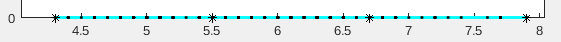
\includegraphics[scale=0.8]{figs/ewd_fisheriris_col1.png}
        \caption{Discretização EWD de acordo com a amostra da tabela \ref{tab:amostraDiscret}}%\footnotemark } 
        \label{fig:faixasFihseririsExemploEWD}
\end{figure}

A partir dos cálculos é definido as seguintes faixas de tamanhos iguais:
\begin{itemize}[noitemsep]
 \item Faixa 1 - [4.3,5.5]
 \item Faixa 2 - ]5.5,6.7]
 \item Faixa 3 - ]6.7,7.9]
\end{itemize}


\subsection{Equal Frequence Discretization - EFD}\label{cap:refTeor:subsec:efd}

Esse outro método de discretização, discretização por frequência iguais do inglês - Equal Frequence Discretization - EFD, já possui uma abordagem diferente do EWD, pois a ideia é manter a quantidade de elementos distintos entre os pontos de corte com o mesmo número \cite{Baron2016,Yang2002}. Dado um intervalo ${[a,b]}$, o número de faixas ${R}$ e a quantidade de valores distintos ${\xi}$ , em que ${\xi \geqslant R}$, o método EFD irá segmentar em ${R}$ faixas de valores que possuem a mesma quantidade de elementos distintos ${\lambda}$. Então serão realizados ${R-1}$ pontos de corte gerando ${R}$ faixas de valores, ${(r_1,...,r_R)}$, com a mesma quantidade de elementos distintos ${\lambda}$. Para encontrar ${\lambda}$ , calcula-se o valor inteiro da divisão entre a quantidade de elementos distintos ${\xi}$ pela quantidade de faixas de valores ${R}$, obtendo o número de elementos da faixa (equação \ref{eq:qtdelemfaixaEFD}). 
\begin{equation}
\lambda = \frac{\xi}{R}
 \label{eq:qtdelemfaixaEFD}
\end{equation}
\begin{itemize}[noitemsep]
 \item ${\lambda}$ - número de elementos da faixa
 \item ${R}$ - total de elementos distintos nas faixas
 \item ${\xi}$ - número de faixas
\end{itemize}


Uma observação nesse método é a ocorrência de uma má distribuição de valores entre as faixas, portanto, caso haja um número significativo de valores repetidos de um atributo, isso causa um desequilíbrio na distribuição dos elementos dentro da faixa. Essa situação reflete em faixas com muitos valores e outras sem nenhuma. 

Uma vez no intervalo ${[a,b]}$ de elementos ordenados e calculado ${\lambda}$ contendo ${R}$ elementos em um vetor ${v_{[R]}}$, tem-se os pontos de corte ${(c_1,...,c_{R-1})}$ como  delimitadores das faixas. Cada ponto de corte ${c_i}$ pode ser calculado por ${v_{i\lambda}-ésimo}$ elemento (equação \ref{eq:pontocorteEFD}).

A equação \ref{eq:pontocorteEFD} é responsável pelo ponto de corte da faixa:
\begin{equation}
c_i = v_{[i\lambda]}
 \label{eq:pontocorteEFD}
\end{equation}
\begin{itemize}[noitemsep]
 \item ${c_i}$ - iésimo ponto de corte
 \item ${R}$ - total de elementos distintos nas faixas
 \item ${\xi}$ - quantidade de faixas de valores
\end{itemize}

Igual ao que aconteceu no método EWD, o valor que estiver no intervalo ${[a,c_1]}$ terá seu valor associado a um valor discreto igual ao índice ${i}$ de sua faixa ${r_i}$, conforme figura \ref{fig:faixasEFD} que exibe as  faixas (${r}$) de tamanhos variáveis no intervalor ${[a,b]}$. Então, caso o valor esteja na faixa ${r_2}$, ele passará a ter o valor de seu índice ${i}$ igual a ${2(dois)}$. De maneira consecutiva, os valores que estiverem na faixa ${r_3=]c_2,c_3]}$ terão valor 3 (três). Uma outra observação desse método é que, diferente do EWD, os intervalos podem assumir faixas com tamanhos diferentes.

%\afterpage{
\begin{figure}[h]
        \centering
        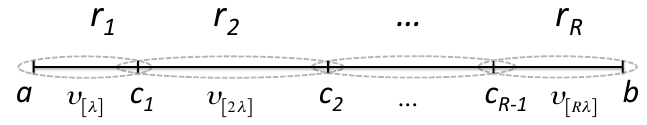
\includegraphics[scale=0.6]{figs/discretizacaoEFD.png}
        \caption[Discretização EFD]{Discretização EFD. Figura baseada em \cite{Lopes2016}} 
        \label{fig:faixasEFD}
\end{figure} 
%\footnotetext{Figura extraída de \cite{LOPES2014}}
%}

Neste exemplo com o método EFD, exibido o resultado na figura \ref{fig:faixasFihseririsExemploEFD}, a tabela \ref{tab:amostraDiscret} também é utilizada na disposição dos valores em cada faixa, bem como o cálculo de ${\lambda}$ (equação \ref{eq:qtdelemfaixaEFD}), que é a divisão do total  de elementos distintos (${\xi}$) pelo o número de faixas ${R=3}$. Após tal cálculo, é realizado a ordenação dos valores, e uma  vez os valores ordenados, soma-se o valor mínimo com ${\lambda}$, encontrando ${c_1}$  como primeiro ponto de corte, e assim sucessivamente, para os outros pontos de corte (${c_2=c_1+\lambda}$), até ${R-1}$ pontos de corte. Na figura \ref{fig:faixasFihseririsExemploEFD} pode-se perceber como a distribuição  dos valores da amostra se comportam no método EFD. Os asteriscos delimitam o início e fim de cada faixa de valor, e os pontos são os valores propriamente ditos.

Neste exemplo com o método EFD, exibido o resultado na figura \ref{fig:faixasFihseririsExemploEFD}, a tabela \ref{tab:amostraDiscret} também é utilizada na disposição dos valores em cada faixa, bem como o cálculo de ${\lambda}$ (equação \ref{eq:qtdelemfaixaEFD}), que é a divisão do total de elementos distintos (${\xi}$) pelo  número de faixas ${R=3}$. Após tal cálculo, é realizada a ordenação dos valores e, uma vez os valores ordenados, soma-se o valor mínimo com ${\lambda}$, encontrando ${c_1}$ como primeiro ponto de corte e assim sucessivamente para os outros pontos de corte (${c_2=c_1+\lambda}$) até ${R-1}$ pontos de corte. Na figura \ref{fig:faixasFihseririsExemploEFD}, pode-se perceber como a distribuição dos valores da amostra se comportam no método EFD. Os asteriscos delimitam o início e fim de cada faixa de valor e os pontos são os valores propriamente ditos. 

\begin{figure}[h] 
        \centering
        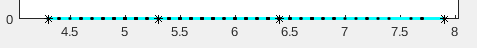
\includegraphics[scale=0.9]{figs/efd_fisheriris_col1.png}
        \caption{Discretização EFD de acordo com a amostra da tabela \ref{tab:amostraDiscret}}%\footnotemark } 
        \label{fig:faixasFihseririsExemploEFD}
\end{figure}

O número de elementos distintos na amostra de dados da tabela \ref{tab:amostraDiscret} é de 35 (trinta e cinco) elementos e dividindo-se por ${R=3}$, que é o número de faixas, encontrar-se-á ${\lambda=11}$. Na lista de números distintos o 11º (décimo primeiro) elemento a partir de ${a}$ (menor valor da amostra) será o primeiro ponto de corte (${c_1}$). Então, todos os valores de ${4,3}$ a ${5,3}$ (identificados por asterisco) fazem parte da primeira faixa.

A seguir são definidas as faixas, percebendo-se que são de tamanhos diferentes ao do método EWD, pois há valores repetidos:

\vspace{-3mm}
\begin{itemize}[noitemsep]
 \item Faixa 1 - [4.3,5.3]
 \item Faixa 2 - ]5.3,6.4]
 \item Faixa 3 - ]6.4,7.9]

\end{itemize}


 

\section{Trabalhos Correlatos}\label{cap:refTeor:sec:trabcorrel}

Esta seção propõe relacionar outros trabalhos, servindo de complemento teórico envolvendo assuntos como: agrupamentos de dados, aprendizado de máquina, classificação e rotulação de dados. 

Em \cite{Jirasirilerd2018}, os autores fazem uso de rotulação automática de textos em Tailandês retirados de notícias da internet. É utilizado para classificar esses textos com a devida categoria (TI, entretenimento, astronomia, etc). Essa pesquisa utiliza para rotulação vetor de representação de documentos e na separação das palavras Tailandesas é aplicado algoritmo de \textit{Convolutional Neural Network} (CNN). Então o modelo faz: i) Conversão de parágrafos e palavras para os vetores utilizando a técnica de representação distribuída; ii) extrai vetores com parágrafos semelhantes; iii) cria um vetor de características; iv) extrai vetores com palavras semelhantes; v) rotula.
%--- textuais ---



Em \cite{Yeganova2010} é utilizada a ideia de dados naturalmente rotulados em uma abordagem que faz detecção e identificação de abreviações na literatura biomédica utilizando aprendizado de máquina supervisionado. Por meio dos textos é realizada uma extração de estruturas textuais (formas curtas, formas longas, formas curtas potenciais e formas longas potenciais), que quando são extraídas naturalmente em pares \textit{i.g.} (forma curta - forma forma longa), (formas curtas potenciais - formas longas potenciais) são tratadas como exemplos positivos. 

Nesse artigo, \cite{Chen2011} se propõe à criação de \textit{clusters} a partir de textos e documentos através de uma abordagem eficaz de agrupamento de documentos, \textit{Fuzzy Frequent Itemset-based Document Clustering} (F2IDC), que combina a mineração de regras de associação \textit{fuzzy} com conhecimento da WordNet. A WordNet é um banco de dados léxico em inglês que agrupa palavras (substantivos, verbos, adjetivos, advérbios) em conjunto de sinônimos e tem com isso o objetivo de melhorar a qualidade dos grupos através dos relacionamentos semânticos. 
 
Nos trabalhos acima citados \cite{Jirasirilerd2018,Yeganova2010,Chen2011} acontecem processos de agrupamentos e rotulação em textos, sendo um tema bastante estudado e diferente desta dissertação, que utiliza o conceito de rotulação de dados no contexto do significado ao grupo formado. 
%-----



O artigo em \cite{Gan2013}  propõe aprendizado de máquina semisupervisionado, que combina agrupamento e classificação com os devidos algoritmos \textit{Fuzzy C-Means} e \textit{SVM} respectivamente. A pesquisa utiliza dados rotulados e não rotulados, apostando na análise do \textit{cluster} como diferencial para compensar a limitação de dados não rotulados e através do conhecimento adquirido melhorar o treinamento do classificador. Essa pesquisa \cite{Gan2013}, diferente desta dissertação, não envolve a interpretação dos grupos após sua formação.

Outro trabalho de agrupamento de dados pode ser visto em \cite{Sun2011}, no qual ele aborda o problema de agrupamento de dados e propõe um algoritmo híbrido com o \textit{support vector cluster} e \textit{K-Means}, ambos de aprendizagem não- supervisionada. Em uma primeira etapa é utilizada uma abordagem do \textit{support vector cluster} com o objetivo de identificar os \textit{outliers} e os pontos sobrepostos e na segunda etapa obtêm-se os núcleos removendo os \textit{outliers} e os pontos sobrepostos e aplicando o \textit{K-Means} nos núcleos para obter o conjunto de dados em \textit{clusters}. Foram utilizadas algumas variáveis de extrema importância para conclusão do trabalho e essas variáveis foram configuradas empiricamente em fases diferentes a fim de obter bons resultados nos agrupamentos de dados. O estudo desse trabalho é interessante no conceito da formação de bons grupos de dados, pois em rotulação de grupos há uma correlação de grupos bem definidos e bons rótulos.

Outro artigo, o autor \cite{Iwamura2013}, faz rotulação automática de textos de cenas em uma base de dados. São textos que se encontram em uma imagem, \textit{e.g.}, uma imagem da fachada de uma casa que possui um número de identificação. O modelo utiliza imagens contendo caracteres, segmenta essas imagens e, após, classifica o caractere através de uma base de dados com várias amostras armazenadas, fazendo seu reconhecimento. Fica claro que esse artigo faz rotulação, mas não da mesma forma definida nesta dissertação, a qual faz uso de aprendizado de máquina a fim de rotular grupos e dando significado a eles. 

%Já no seguinte artigo \cite{Majid2016} o autor utiliza um algoritmo de aprendizado supervisionado, Support Vector Machine - SVM, para identificar através de imagens de satélite (WorldView-3) quais tipos de árvores dominantes estão em determinada região através de técnica de classificação. Isto posto,   os dados do inventário de árvores foram sistematicamente divididos entre teste de amostra e conjunto de dados de validação. 

O trabalho \cite{Costa2016} utiliza classificação não-supervisionada, mas possui uma característica diferenciada por utilizar dados \textit{online}. O método faz uso da aprendizagem a partir de uma base de regras vazias com o processamento das amostras desses dados online e não é necessário pré-definir parâmetros iniciais e nem número ou tamanho das classes. Efetivamente, o autor foca em conceito-evolução, portanto, o algoritmo se adapta continuamente para lidar com mudanças de dados que podem surgir ao se lerem novas amostra de dados. Essa abordagem não-supervisionada conta com o conceito de \textit{Typicality and Eccentricity Data Analytics} (TEDA), utilizado em problemas no mundo real como detecção de falhas; no entanto, mesmo sendo um comportamento não-supervisionado, em vez de \textit{clusters} tradicionais, o algoritmo trabalha com conceito de nuvens de dados. Nesta dissertação a utilização da rotulação são para grupos já formados, diferente dessa pesquisa, que possui o objetivo da formação dinâmica de grupos.



O trabalho proposto por \citeonline{Lopes2016} faz um estudo abordando o tema de rotulação de dados conforme definição  \ref{teo:lopes:problema}.
% 
%\newtheorem{teorema}{Definição}
    \begin{teorema}
Dado um conjunto de \textit{clusters} ${C=\{c_1,...,c_k | K \geqslant 1\} }$, de modo que cada cluster contém um conjunto de elementos ${c_i=\{\vec{e}_1,..,\vec{e}_{n^{(c_i)}}|n^{(c_i)} \geqslant 1 \}}$ que podem ser representados por um vetor de atributos definidos em ${\mathbb{R}^m }$ e expresso por ${ \vec{e}^{c_i}=(a_1,..,a_m)  }$ e ainda que  com ${ c_i \cap c_{i'}=\emptyset }$ com ${ 1 \leqslant i, i \leqslant K  }$ e ${ i \neq i' }$; o objetivo consiste em apresentar um conjunto de rótulos ${ R=\{ r_{c1},...,r_{ck} \} }$, no qual cada rótulo específico é dado por um conjunto de pares de valores, atributo e seu respectivo intervalo, ${ r_{ci}=\{ (a_1,[p_1,q_1]),...,(a_{m^{(c_i)}}, ]p_{m^{(c_i)}},q_{m^{(c_i)}}]) \} }$ capaz de melhor expressar o cluster ${c_i}$ associado.
        %\footnotemark 
        %\footnotetext{Definição retirada de \cite{LOPES2014}}
        \begin{itemize}[noitemsep]
            \item ${K}$ é o número de \textit{clusters};
            \item ${c_i}$ é o i-ésimo \textit{cluster};
            \item ${n^{c_i}}$ é o número de elementos do \textit{cluster} ${c_i}$;
            \item ${\vec{e}_{j^{(c_i)}}}$ se refere ao j-ésimo elemento pertencente ao \textit{cluster} ${c_i}$;
            \item ${m}$ é a dimensão do problema;
            \item ${r_{c_i}}$ é o rótulo referente ao \textit{cluster} ${c_i}$;
            \item ${]p_{m^{(c_i)}},q_{m^{(c_i)}}]}$ representa o intervalo de valores do atributo ${a_{m^{(c_i)}} }$, onde ${ p_{m^{(c_i)}} }$  é o limite inferior e ${ q_{m^{(c_i)}} }$ é o limite superior;
        \end{itemize}
    \label{teo:lopes:problema}
    \end{teorema}


O estudo utilizou como entrada um conjunto de dados em que foi realizado o agrupamento com algoritmos não-supervisionados para formação de \textit{clusters} e logo após a formação destes, é utilizado um algoritmo supervisionado (RNA) nos grupos de dados já discretizados e apresentado como saída um rótulo específico que melhor define o grupo formado. 

Os rótulos são formados por uma tupla, atributos mais relevantes e faixa de valores que mais se repetem. A figura \ref{fig:modeloLOPES} representa o modelo de atuação do autor citado, que por meio de 4 passos (I, II, III, IV),  obtiveram-se os rótulos que representaram os \textit{clusters}. 
\begin{figure}[h]
        \centering
        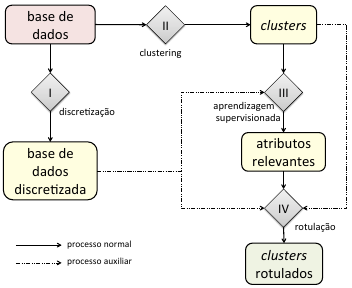
\includegraphics[scale=1]{figs/modeloLopes.png}
        \caption{Modelo de \cite{Lopes2016}} 
        \label{fig:modeloLOPES}
\end{figure}

Em analogia a este trabalho na figura \ref{fig:modeloLOPES}, em que é aplicado o algoritmo de RNA, o processo III é o local exato que esta pesquisa utiliza para testar a visibilidade de outros algoritmos supervisionados. Nesse modelo proposto, o autor não só tem a preocupação de processar a formação dos grupos como também aplicar um algoritmo supervisionado para rotular esses grupos formados. Já nesta dissertação, o foco é fazer testes em grupos já definidos utilizando algoritmos supervisionados com paradigmas  ainda não testados, e apresentar os rótulos encontrados. Deixando claro que a utilização de grupos já classificados foi necessária para essa pesquisa para mostrar a acurácia, número de registros representados pelo rótulo, mas a aplicação deste estudo tem aplicabilidade nos grupos não classificados a fim de encontrar rótulos que identifiquem  grupos.



Em \citeonline{Metodo2015,DeLima2015} são trabalhos que tem como objetivo principal a rotulação de grupos de dados, mas no primeiro trabalho o autor utiliza uma técnica de aprendizado semisupervisionada, que visa fazer rotulação de dados através de uma pequena amostra rotulada. Em \citeonline{DeLima2015} é aplicada rotulação a uma base de dados de uma rede social chamada de Scientia.Net, com o objetivo na criação de grupos e identificação dos atributos que podem ser importantes ao ponto de representar estes grupos, chamando-os de rótulos. Nesse artigo, o autor utilizou o modelo de \cite{Lopes2016} para rotulação de dados com os mesmos algoritmos, o  \textit{k-means} para agrupamento, e logo na segunda parte a utilização do algoritmo supervisionado, \textit{Artificial Neural Networks} - ANN. Diferente dos trabalhos \cite{Metodo2015,DeLima2015}, este trabalho proposto tem o foco em testes somente nos algoritmos supervisionados nos grupos já formados de acordo com a origem da base de dados, a fim de gerar rótulos e assim, aferir suas acurácias para cada um desses algoritmos testados. 
% O trabalho de \citeonline{Metodo2015} é baseado em fazer a classificação e rotulação em uma base que possuem poucos elementos classificados utilizando método semisupervisionado. Na aprendizagem de máquina semisupervisionada o foco é quando não há muitos exemplos em quantidade suficientes ao ponto de conseguir treinar um classificador que desempenhe bem seu papel. 
% 
% O autor aplica a combinação de um classificador e um agrupador para desempenhar  a tarefa de classificação dos dados baseando-se nos algoritmos co-training e $k-means_ki$.
% 
% 
% O método inicia com uma base dividida em elementos classificados (L) e não classificados (U). Após cada iteração o grupo L vai crescendo e automaticamente diminuindo o grupo U até que não tenha mais nenhum elemento em U, figura  \ref{fig:modeloVicente}. Após isso é realizado uma etapa de agrupamento, sem levar em consideração os dados classificados anteriormente. Terminada essa etapa é feito uma validação para saber quais os rótulos foram considerados corretos.
% \begin{figure}[!h]
%         \centering
%         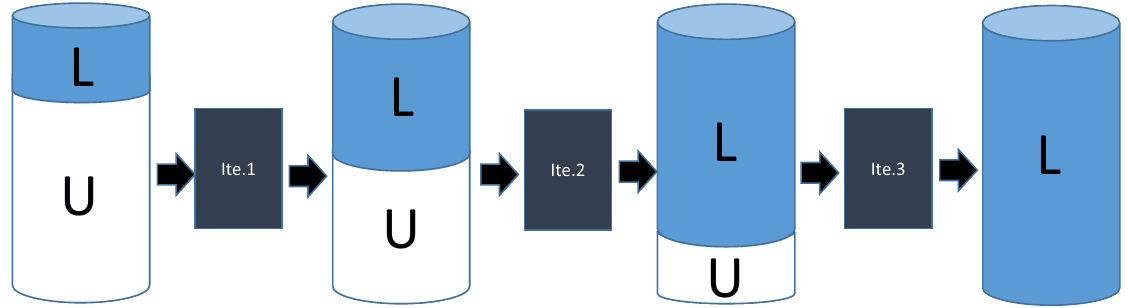
\includegraphics[scale=0.4]{figs/modeloVicente.png}
%         \caption{Comportamento da base de dados a cada iteração. Método \cite{Metodo2015}} \label{fig:modeloVicente}
% \end{figure}
% 
% O método proposto é uma combinação de um classificador com um método de agrupamento, onde a rotulação de um conjunto de dados é feita com conhecimento prévio de um outro conjunto menor rotulado. O classificador treina com a parte de dados rotulada e classifica os dados não-rotulados.

Outra pesquisa \cite{Filho2015}  aborda o mesmo problema de rotulação, mas com atuação diferente, pois o modelo utiliza o algoritmo não-supervisionado \textit{Fuzzy C-Means} para composição dos grupos, em que o número de grupos é fornecido na inicialização do algoritmo e também na definição das faixas de valores de atributos de cada atributo rótulo do grupo formado. A diferença entre esta dissertação e esse artigo de \citeonline{Filho2015} é o modelo de resolução, que utiliza somente o algoritmo \textit{Fuzzy C-Means} para criar os grupos e definir as faixas de valores de cada atributo rótulo e também a ausência da técnica de discretização dos valores dos dados para obter os rótulos.



%Outra pesquisa \cite{Filho2015}  aborda o mesmo Problema de Rotulação, mas a atuação é diferenciada, pois o modelo procura diferenças existentes em cada grupo através da seleção dos elementos que representam o grupo, e depois é construído a faixa de valores. Os grupos são formados pelo algoritmo Fuzzy C-Means e após isso que é selecionado os atributos. Através do algoritmo Fuzzy C-Means é criada uma tabela chamada de matriz U, ou matriz de partição \textit{fuzzy}. Essa matriz contém um número relacionado a cada grupo chamado, Grau de Pertinência - GP, onde este número varia de 0 a 1 dependendo do grau de proximidade com o centróide de um grupo. Quanto mais próximo ao centróide, maior é seu grau de pertinência em relação ao grupo. Através dessa tabela criada com os valores de pertinência são escolhidos os atributos que farão parte de cada grupo. A cada atributo é verificado o GP de cada grupo, e o atributo pertencerá ao grupo que tiver o maior GP. Isso significa que quanto maior o valor de GP, mais próximo do centróide do grupo, consequentemente, mais pertencente ao grupo. 

%Nesse modelo proposto pelo autor \cite{Filho2015} existem duas variáveis onde são atribuídos parâmetros: Grau de Seleção - GS e Incremento do Grau de Seleção - IGS. O GS, serve de base para seleção dos elementos mais significativos na formação do rótulo e o IGS seria um incremento do parâmetro GS, sendo que, tanto GS quanto IGS podem variar de 0 a 1. Esses parâmetros são inicializados no início do modelo de resolução e são incrementados a cada iteração, que ocorre caso não exista pelo menos uma faixa de valor pertencente a cada grupo. A forma de medir a acurácia do autor \cite{Filho2015} coincide com este trabalho, pois são utilizados os grupos já predefinidos pelo autor da base de dados de exemplo, e dessa forma ao se refazer os novos grupos pode-se comparar com os grupos originais e verificar os resultados do modelo e aferir a acurácia dos rótulos de cada grupo. 


Outro autor  \citeonline{Imperes2018a} em seu trabalho utiliza uma proposta de rotulação semelhante a outra pesquisa \citeonline{Filho2015}, mas com outro algoritmo, \textit{K-means} não-supervisionado, baseado em distância. Esse modelo é constituído de duas etapas, sendo a primeira a transformação da distância gerada pelo \textit{K-means} em GP, e logo após, na segunda etapa, é realizada a rotulação de dados de acordo com a tabela gerada na primeira etapa. São feitas várias iterações até encontrar faixas únicas de valores para cada atributo rótulo. Ao se comparar esta dissertação com a pesquisa desse autor \cite{Imperes2018a}, percebe-se que também não há um processo de discretização de valores dos atributos e também não há aplicação de dois algoritmos de aprendizado. 

%Outro autor \cite{imperes2018} utilizou em seu trabalho  uma proposta de rotulação com o algoritmo não-supervisionado, \textit{K-means}, que é baseado em distância, e desenvolveu em seu método a transformação da saída padrão, em distância, para que cada elemento da base de dados recebesse um GP. Esse GP é utilizado para selecionar os elementos relevantes em cada grupo. Esse modelo funciona em duas etapas, a primeira transforma as saídas em distâncias para GP, e a segunda etapa, formar as faixas de valores e exibir os rótulos. No início da primeira etapa são atribuídos os parâmetros do números de grupos, GP, GS e IGS, após, é carregado a base de dados e formados os grupos através de algoritmo baseado em distância (\textit{K-means}). Logo em seguida a transformação da saída de distância em GP, por conseguinte os grupos já ficam atuliazados contendo GP. Na segunda etapa acontece a seleção dos elementos a partir da comparação do GP e do GS, portanto em seguida, a escolha do menor e maior valor do atributo formando a faixa de valor. Caso haja pele menos uma faixa de valor pertencente a cada grupo os rótulos são exibidos, mas caso não ocorra, GS é incrementado pelo IGS refazendo a segunda etapa novamente. 

No trabalho de rotulação \citeonline{araujo2017} defende que uma etapa de fundamental importância para se ter bons resultados na rotulação de grupos de dados se dá na clusterização. Portanto, quanto mais eficiente for a técnica de agrupamento de dados utilizada, maior será acurácia dos grupos encontrados. A partir do que foi dito, o autor utiliza o DAMICORE no método de rotulação automática para criar grupos. DAMICORE é um método de detecção de correlação de dados e tem como característica a não informação do número de \textit{clusters} ao qual o algoritmo é aplicado. O modelo é dividido em cinco etapas até se obterem os rótulos. A etapa I e II preparam os dados e ajudam a medir a similaridade dos elementos, oferecendo uma maior precisão e contribuindo para criação de grupos mais significativos. Na etapa III ocorre a clusterização, e como não é preciso informar o número de \textit{cluster} na utilização do DAMICORE, os resultados nesta etapa acabam por superar um número razoável de \textit{clusters} para uma melhor compreensão e, em razão disso, a etapa IV, de mesclagem, faz a junção de \textit{clusters} para criação de \textit{super-clusters}, que são \textit{clusters} maiores representando um conceito mais geral e de mais fácil entendimento. Por fim, os \textit{super-clusters} são submetidos ao método de rotulação automática na etapa V, permitindo identificar os atributos mais relevantes e suas respectivas faixas de valores. Essa pesquisa mantém o foco na etapa de formação dos \textit{clusters} e se diferencia do texto desta dissertação exatamente nisso, pois nesta dissertação é pressuposto que os grupos testados são \textit{clusters} bem definidos e classificados, posto que este trabalho não cria grupos e sim os utiliza. 

%Nas pesquisas realizadas a cerca do tema de ``rotulação de grupos'', foi encontrado vários trabalhos que em seus títulos possuia a palavra ``rotulaçao'', mas não no sentido empregado aqui, nesta pesquisa - a exemplo dentre esses vários trabalhos encontrados, o autor \cite{} faz a rotulação de objetos, cujo problema abordado é a leitura de identificadores de objetos em forma de rolo de ``papel bolha'', onde há dificulta do leitor lêr os rótulos dos rolos em uma esteira, pois não há condições de prever qual posição estára o identificador do objeto ao chegar no leitor. Isso mostra que referente ao tema desta pesquisa   (Citar aqui vários trabalhos de 2017,2018)
